% Options for packages loaded elsewhere
\PassOptionsToPackage{unicode}{hyperref}
\PassOptionsToPackage{hyphens}{url}
\PassOptionsToPackage{dvipsnames,svgnames,x11names}{xcolor}
\documentclass[
  11pt,
  a4paper,
]{article}
\usepackage{xcolor}
\usepackage[margin=24mm]{geometry}
\usepackage{amsmath,amssymb}
\setcounter{secnumdepth}{-\maxdimen} % remove section numbering
\usepackage{iftex}
\ifPDFTeX
  \usepackage[T1]{fontenc}
  \usepackage[utf8]{inputenc}
  \usepackage{textcomp} % provide euro and other symbols
\else % if luatex or xetex
  \usepackage{unicode-math} % this also loads fontspec
  \defaultfontfeatures{Scale=MatchLowercase}
  \defaultfontfeatures[\rmfamily]{Ligatures=TeX,Scale=1}
\fi
\usepackage{lmodern}
\ifPDFTeX\else
  % xetex/luatex font selection
  \setmainfont[BoldFont=texgyrepagella-bold.otf,ItalicFont=texgyrepagella-italic.otf,BoldItalicFont=texgyrepagella-bolditalic.otf]{texgyrepagella-regular.otf}
  \setmonofont[BoldFont=lmmonolt10-bold.otf]{lmmono10-regular.otf}
  \setmathfont[]{texgyrepagella-math.otf}
\fi
% Use upquote if available, for straight quotes in verbatim environments
\IfFileExists{upquote.sty}{\usepackage{upquote}}{}
\IfFileExists{microtype.sty}{% use microtype if available
  \usepackage[]{microtype}
  \UseMicrotypeSet[protrusion]{basicmath} % disable protrusion for tt fonts
}{}
\makeatletter
\@ifundefined{KOMAClassName}{% if non-KOMA class
  \IfFileExists{parskip.sty}{%
    \usepackage{parskip}
  }{% else
    \setlength{\parindent}{0pt}
    \setlength{\parskip}{6pt plus 2pt minus 1pt}}
}{% if KOMA class
  \KOMAoptions{parskip=half}}
\makeatother
\usepackage{longtable,booktabs,array}
\usepackage{caption}
\captionsetup[table]{skip=6pt}
\newcounter{none} % for unnumbered tables
\usepackage{calc} % for calculating minipage widths
% Correct order of tables after \paragraph or \subparagraph
\usepackage{etoolbox}
\makeatletter
\patchcmd\longtable{\par}{\if@noskipsec\mbox{}\fi\par}{}{}
\makeatother
% Allow footnotes in longtable head/foot
\IfFileExists{footnotehyper.sty}{\usepackage{footnotehyper}}{\usepackage{footnote}}
\makesavenoteenv{longtable}
\usepackage{graphicx}
\makeatletter
\newsavebox\pandoc@box
\newcommand*\pandocbounded[1]{% scales image to fit in text height/width
  \sbox\pandoc@box{#1}%
  \Gscale@div\@tempa{\textheight}{\dimexpr\ht\pandoc@box+\dp\pandoc@box\relax}%
  \Gscale@div\@tempb{\linewidth}{\wd\pandoc@box}%
  \ifdim\@tempb\p@<\@tempa\p@\let\@tempa\@tempb\fi% select the smaller of both
  \ifdim\@tempa\p@<\p@\scalebox{\@tempa}{\usebox\pandoc@box}%
  \else\usebox{\pandoc@box}%
  \fi%
}
% Set default figure placement to htbp
\def\fps@figure{htbp}
\makeatother
\setlength{\emergencystretch}{3em} % prevent overfull lines
\providecommand{\tightlist}{%
  \setlength{\itemsep}{0pt}\setlength{\parskip}{0pt}}
\usepackage{mathtools}
\usepackage{graphicx}
\usepackage{needspace}
\usepackage{xurl}
\usepackage{etoolbox}
\usepackage{fancyhdr}
\usepackage{titlesec}
\setlength{\parindent}{0pt}
\setlength{\parskip}{5.5pt plus 1pt minus 1pt}
\setlength{\emergencystretch}{2em}
\clubpenalty=10000
\widowpenalty=10000
\displaywidowpenalty=10000
\raggedbottom
\pagestyle{fancy}
\fancyhf{}
\fancyfoot[C]{\small\thepage}
\renewcommand{\headrulewidth}{0pt}
\titleformat{\section}{\normalfont\Large\bfseries}{}{0pt}{}
\titlespacing*{\section}{0pt}{16pt plus 3pt minus 2pt}{7pt}
\pretocmd{\section}{\Needspace{6\baselineskip}}{}{}
\pretocmd{\subsection}{\Needspace{5\baselineskip}}{}{}
\makeatletter
\renewenvironment{figure}[1][]{\par\noindent\begin{minipage}{\linewidth}\def\@captype{figure}}{\end{minipage}\par\medskip}
\def\@maketitle{\newpage\null\begin{center}{\LARGE\bfseries\@title\par}\vskip .9em{\large\@author\par}\vskip .5em{\small\@date\par}\end{center}\vskip .4em}
\makeatother
\newsavebox{\papereqbox}
\newcommand{\paperdisplay}[2][]{\par\begingroup
\sbox{\papereqbox}{$\displaystyle #2$}
\typeout{PAPER-EQUATION-WIDTH: \the\wd\papereqbox; available \the\linewidth; tag #1}
\begin{equation*}\ifdim\wd\papereqbox>.93\linewidth
\resizebox{.93\linewidth}{!}{\usebox{\papereqbox}}\else\usebox{\papereqbox}\fi
\ifstrempty{#1}{}{\tag{#1}}\end{equation*}\endgroup\par}

\usepackage{bookmark}
\IfFileExists{xurl.sty}{\usepackage{xurl}}{} % add URL line breaks if available
\urlstyle{same}
% fallback for those not using the hyperref driver hyperxmp:
\makeatletter
\@ifundefined{xmpquote}{\newcommand{\xmpquote}[1]{#1}}{}
\makeatother
\hypersetup{
  pdftitle={Tri-Octagon Reference-Scaffold Geometry: Exact Construction of an Alternating Hexagonal Core},
  pdfauthor={Hilmir Frímann Halldórsson},
  colorlinks=true,
  linkcolor={MidnightBlue},
  filecolor={Maroon},
  citecolor={Blue},
  urlcolor={MidnightBlue},
  pdfcreator={LaTeX via pandoc}}

\title{Tri-Octagon Reference-Scaffold Geometry: Exact Construction of an Alternating Hexagonal Core}
\author{Hilmir Frímann Halldórsson}
\date{Paper D · Revision v0.1.1 · 23 September 2026}

\begin{document}
\maketitle

\section{Abstract}\label{abstract}

Three regular octagons can serve as geometric reference frames without being interpreted as a connected material shell. This paper formalizes an author-clarified construction in which three selected octagon edges alternate with three deliberately added connectors. In an explicitly aligned \(C_3\) family, an edge has length \(s>0\), its midpoint lies at radius \(p\), and the connector length is \(g_{\mathrm{gap}}=\sqrt3p-s/2>0\). The resulting chain is a convex equiangular hexagon with alternating lengths \((s,g_{\mathrm{gap}},s,g_{\mathrm{gap}},s,g_{\mathrm{gap}})\). It is regular exactly when \(g_{\mathrm{gap}}=s\), or \(p=\sqrt3s/2\). An equilateral support triangle of side \(s+2g_{\mathrm{gap}}\) contains three equilateral corner cells of side \(g_{\mathrm{gap}}\); removing those corners gives the hexagon. Complete octagonal reference figures are constructed explicitly.

The top measurement polygon of the separately specified Paper-C welded module belongs to this same aligned family at \(g_{\mathrm{gap}}/s=1/\sqrt2\). Outward translation at fixed face size or shrinkage about fixed vertical face centres reaches the regular condition, but removes the original seams. For an original width-one module, the shrink operation gives six sides of exactly \(1/3\) and lowers the top height. The regular unmarked hexagon has \(D_6\) symmetry, while the edge/connector role marking retains \(D_3\). A bounded source trace relates historical Z-vector and torus displays to their actual state inputs and consumers. Their attachment to the clarified gap cells remains unspecified. The paper separates author testimony, historical statements, exact mathematics, conditional geometric comparisons and open model interfaces. It introduces no dynamics or physical energy law.

\textbf{Preparation and provenance.} Author and design clarification: Hilmir Frímann Halldórsson. Mathematical formalization, source tracing, figures and preparation: Codex, with GPT as scientific lead. Version history and the scoped scientific-review disposition are recorded in the accompanying package.

\section{1. Introduction}\label{introduction}

An octagon can be a polygonal region, a wire frame, an ordered list of directions, a coordinate reference, or one face of a three-dimensional surface. These uses share elementary geometry but impose different mathematical requirements. A material surface may require adjacency and boundary conditions. A reference frame need only provide reproducible points, directions and scales. A curve constructed from those references can remain well defined after the octagons themselves have been hidden from a display.

This distinction is central to the Tri-Octagon reconstruction. Historical research used octagonal figures alongside projected root systems, dual tetrahedra, phase lattices, three-channel recurrences and toroidal displays. Later work specified an exact welded local module, published as Paper C. The repeated name did not establish that every object was one surface in different coordinates. Treating the octagons as necessarily filled physical panels imposed conditions that were not part of the author\textquotesingle s intended reference-scaffold construction.

The author clarified on 23 September 2026 that three selected octagon edges and three straight connectors were intended to define an alternating six-segment structure. Equal selected-edge and connector lengths, together with the intended turning angles, give its regular-hexagon condition. The purpose of this paper is to make that statement precise enough to reconstruct without access to a conversation or an image. The alignment assumptions are therefore as important as the length equality.

The mathematical problem has two continuous parameters before a choice of scale: selected-edge length \(s\) and midpoint radius \(p\). Once tangential alignment is fixed, both the connector direction and its length follow. The dimensionless ratio \(g_{\mathrm{gap}}/s\) is the shape parameter. Setting it to one is a tuning condition, not a consequence of threefold symmetry alone. The derivation below supplies closure, orientation and convexity as well as the more immediately visible equal-angle statement.

The resulting mathematics is elementary Euclidean geometry. No novelty is claimed for regular polygons, support-line constructions or triangular truncation. The contribution is a precise model-specific definition, an explicit relation to the Paper-C measurement polygon, and a separation of those facts from unestablished dynamical and historical identifications. A reader interested only in geometry can follow Sections 4--14 independently. Sections 2--3 give provenance; Sections 15--20 explain the model interfaces and limits; the appendices identify reproducible evidence.

\section{2. Design provenance and levels of evidence}\label{design-provenance-and-levels-of-evidence}

Five evidence levels are used throughout. \textbf{A: historical source statements} are claims or formulas in preserved research papers or code. Reporting one does not prove it. \textbf{B: author clarification} records present design testimony dated 23 September 2026. \textbf{C: current exact derivation} means a mathematical consequence of explicitly stated assumptions. \textbf{D: conditional comparison} identifies two specified constructions under a displayed map, without identifying their entire surrounding models. \textbf{E: open correspondence} denotes a map or hypothesis for which the required definition or proof is absent.

The distinction matters in both directions. A current proof cannot be backdated merely because its result resembles an old sketch. Conversely, failure to find its exact equation in a bounded source examination does not establish that no related idea existed earlier. The accepted formula for \(g_{\mathrm{gap}}\) is classified B+C: author clarification followed by a constructive coordinate formalization. It is not a recovered 2025 equation.

The immediate mathematical source is Section 6 of the accepted \emph{Tri-Octagon Hexagon Core Derivation v0.1} {[}I2{]}. Its assumptions and proof are developed here in full. The lineage report {[}I1{]} records the earlier targeted examination of 46 PDF paths, representing 45 distinct contents; it does not claim that every assertion in those papers was verified. This paper reuses that record. It does not repeat a corpus screen or the earlier proof suites.

The author\textquotesingle s preserved clarification {[}I4{]} identifies the octagons as reference generators. They determine selected points, edge directions, relative scale, connector locations and cyclic roles. Whether one later fills a face, represents a field on it, or treats a gap as a physical domain requires further data. Such an interpretation cannot be inferred from the construction diagram alone. Equally, a reference origin does not make an associated implemented state map causally irrelevant: that question is settled by its inputs, updates and consumers, as discussed in Section 16.

The paper\textquotesingle s figures are newly rendered construction diagrams from exact analytic coordinates. They are not historical simulation images or evidence of transport. The source-provenance manifest binds the inspected source bytes; the reference ledger distinguishes a directly inspected standard reference from historical claims carried through the existing line-by-line reconstruction.

\section{3. A concise historical sequence}\label{a-concise-historical-sequence}

The sequence below concerns identifiable documents and definitions, not discovery priority. Dates in old documents can be inconsistent with later bibliographies. The preserved lineage uses printed dates and one-based PDF page numbers.

On 29 October 2025, \emph{TriOctagon E8--SU3 Geometry} {[}H1{]}, pp. 4--6, proposed three root octets and a projected organization. Page 4 described a connection to an independently motivated folded construction. That statement is evidence that a folding idea preceded or accompanied the document; it does not supply the exact later Paper-C coordinates. Pages 12 and 18 introduced tetrahedral-aperture and E6-related claims whose complete connecting maps remained unspecified.

The 24 November 2025 \emph{Recursive Engines Across Scales} {[}H2{]}, p. 2, equations (1)--(3), gave translated regular octagons and a tilt prescription. Its planar octagons have the same global angular orientation. Their centre locations alone do not impose the covariant edge alignment used in this paper. A tilt-axis direction also leaves an affine hinge location to be specified. Those omissions must not be repaired retrospectively by substituting the present construction.

The same source, pp. 20--22, supplied explicit opposite tetrahedra and a body-diagonal projection. The same-date \emph{Recursive SRG Evolution} {[}H3{]}, p. 26, showed the associated projected triangular overlap. These establish a distinct exact central-core construction with its own scale. A later December source used octagon angular offsets \(0^\circ,+20^\circ,-20^\circ\) as motivation for return channels. Such offsets are not a uniform 24-direction lattice; the two constructions remain separate in {[}I1{]}.

The 2026 local geometry specification and Paper C {[}I5{]} define three finite regular octagons joined along three full seams. Its exact annular surface, rather than an unspecified larger host, is implemented in the modern geometry module. The author clarification of 23 September 2026 then supplied the intended edge/connector reference-scaffold definition. The accepted aligned derivation and the preserved four-page research note followed. The present paper expands that mathematics and its documented interfaces; the short note remains a valid predecessor.

This history admits related stages without asserting a single uninterrupted coordinate lineage. Original construction files named in historical papers, including \texttt{tri.py}, \texttt{center2.py}, \texttt{center3.py} and a Blender construction, were not located by the earlier targeted investigation. Their absence is a provenance limit, not permission to recreate their contents and label them recovered.

\section{4. Regular octagon reference geometry}\label{regular-octagon-reference-geometry}

Let \(s>0\) be the side length of a regular octagon. Denote its circumradius by \(R_{\mathrm{oct}}\), its apothem by \(a\), and the distance between opposite parallel sides by \(w\). Splitting the isosceles triangle subtended by one side gives a right triangle with angle \(\pi/8\) at the centre. Consequently

\paperdisplay[1]{R_{\mathrm{oct}}=\frac{s}{2\sin(\pi/8)},\qquad
a=\frac{s}{2\tan(\pi/8)}=\frac{1+\sqrt2}{2}s,\qquad
w=2a=(1+\sqrt2)s.}

Here \(\tan(\pi/8)=\sqrt2-1\), obtained from the half-angle identity at \(\pi/4\). Thus \(s=w(\sqrt2-1)\). A statement that an octagon has width one is not a statement that its side is one. This distinction is essential in the worked shrink example.

In an orthonormal local coordinate system, a convenient counterclockwise vertex list is

\paperdisplay[2]{\mathcal V_s=\bigl((a,-s/2),(a,s/2),(s/2,a),(-s/2,a),
(-a,s/2),(-a,-s/2),(-s/2,-a),(s/2,-a)\bigr).}

Write the ordered list (2) as \(\mathcal V_s=(v_0,\ldots,v_7)\) and distinguish the filled convex reference region and its outline:

\paperdisplay[2a]{\mathcal O_s=\operatorname{conv}\{v_0,\ldots,v_7\},\qquad
\partial\mathcal O_s=\bigcup_{k=0}^{7}[v_k,v_{k+1}],\quad v_8=v_0.}

Adjacent vertical or horizontal sides have length \(s\). A diagonal side has coordinate increments of magnitude \(a-s/2=s/\sqrt2\), so its length is also \(s\). The vertex list therefore determines the regular octagon with the metrics in (1). Finite-face statements below use the filled set \(\mathcal O_s\); outline and vertex statements use \(\partial\mathcal O_s\) and \(\mathcal V_s\), respectively. This mathematical filling assigns no physical material. The selected-edge and hexagon construction needs only its specified segments.

\begin{figure}
\centering
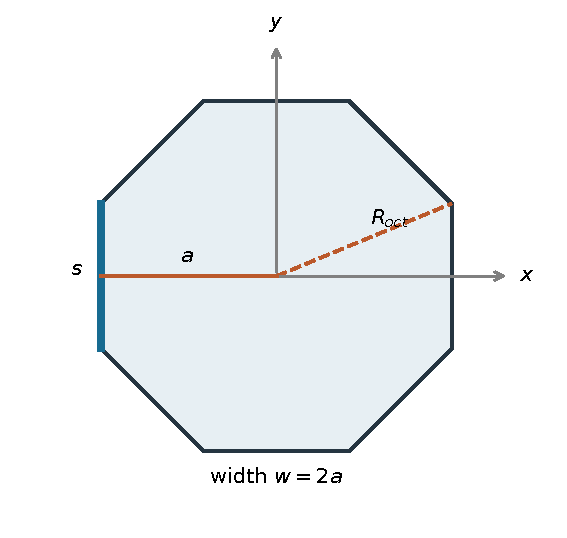
\includegraphics[width=0.78\linewidth,height=\textheight,keepaspectratio,alt={Local regular-octagon geometry. The highlighted inward side has length s; a and R\_\{\textbackslash mathrm\{oct\}\} are different radii. The axes are local reference directions, and the overall width is 2a.}]{figures/01_octagon_metrics.pdf}
\caption{Local regular-octagon geometry. The highlighted inward side has length \(s\); \(a\) and \(R_{\mathrm{oct}}\) are different radii. The axes are local reference directions, and the overall width is \(2a\).}
\end{figure}

The local choice fixes an edge orientation. Rotating a complete octagon without rotating the associated edge convention would change the selected data. In the construction below, the local frame and selected edge rotate together. All lengths may carry an abstract common unit, but no physical calibration is assigned by these equations.

\section{5. Three aligned reference frames}\label{three-aligned-reference-frames}

Fix the origin in the reference plane. For \(i=0,1,2\), with indices understood modulo three, define

\paperdisplay[3]{\phi_i=\frac{2\pi i}{3},\qquad
u_i=(\cos\phi_i,\sin\phi_i),\qquad
t_i=(-\sin\phi_i,\cos\phi_i).}

The vectors \(u_i,t_i\) form a positively oriented orthonormal frame. The first is radial, and \(t_i=Ju_i\) is its counterclockwise quarter-turn. Choose \(p>s/(2\sqrt3)\) and put

\paperdisplay[4]{A_i=p u_i-\frac{s}{2}t_i,\qquad
B_i=p u_i+\frac{s}{2}t_i.}

The segment \(E_i:A_i\to B_i\) has midpoint \(p u_i\) and lies on the support line \(u_i\cdot x=p\). It is tangent to the circle of midpoint radius \(p\). The term tangent refers to this reference circle, not to a motion or an orbit. These three oriented segments are the selected octagon-derived edges.

The explicit inequality on \(p\) is the positive-connector domain. It will make the directed connector coefficient strictly positive. At equality, each connector collapses and the purported hexagon degenerates. Below it, the displayed algebra still produces vectors, but their direction signs and the intended corner-cut interpretation change; those cases are not included in the theorem.

\begin{figure}
\centering
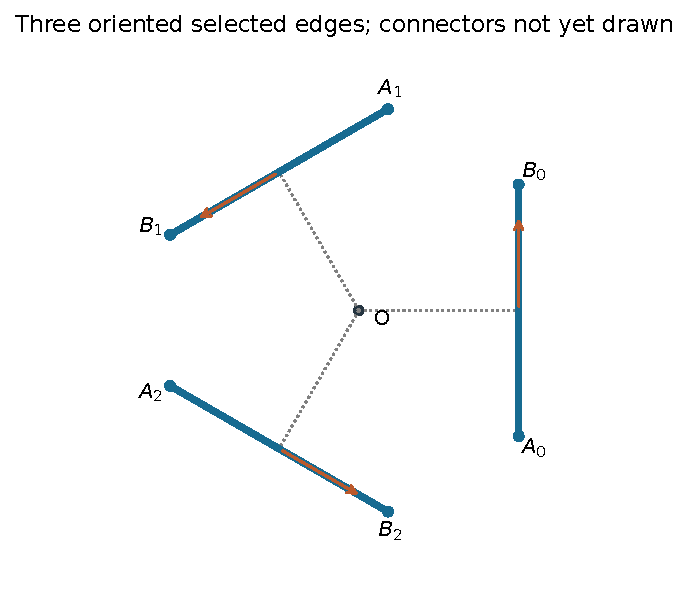
\includegraphics[width=0.78\linewidth,height=\textheight,keepaspectratio,alt={Three selected edges in their radial/tangential frames, before adding connectors. Endpoint labels specify the orientation and therefore remove the ambiguity in joining neighboring edges.}]{figures/02_three_frames.pdf}
\caption{Three selected edges in their radial/tangential frames, before adding connectors. Endpoint labels specify the orientation and therefore remove the ambiguity in joining neighboring edges.}
\end{figure}

The family is \(C_3\)-covariant because rotation by \(2\pi/3\) takes every indexed object to the next. This statement is stronger than placing three centres on an equilateral triangle while keeping all finite octagons at one global orientation. It is also more specific than abstract threefold symmetry: symmetry alone would permit selected edges tilted relative to the tangent directions. Formula (4) is the alignment assumption that makes the following turns exact.

\section{6. Connector lemma and the six-segment chain}\label{connector-lemma-and-the-six-segment-chain}

Define \(G_i:B_i\to A_{i+1}\). The ordered chain is

\paperdisplay[5]{E_0,G_0,E_1,G_1,E_2,G_2,
\qquad (H_0,H_1,H_2,H_3,H_4,H_5)=(A_0,B_0,A_1,B_1,A_2,B_2).}

\textbf{Lemma 1 (directed connector).} Under (3)--(4), with \(R_{60}\) the rotation through \(+\pi/3\),

\paperdisplay[6]{B_i-A_i=s t_i,\qquad
A_{i+1}-B_i=\left(\sqrt3p-\frac{s}{2}\right)R_{60}t_i.}

\textbf{Proof.} The first identity follows by subtracting (4). For the second, the \(i=0\) data are

\paperdisplay[]{u_1-u_0=(-3/2,\sqrt3/2),\qquad t_1+t_0=(-\sqrt3/2,1/2).}

Subtracting the appropriate endpoints gives

\paperdisplay[7]{\begin{aligned}
A_1-B_0
&=p(u_1-u_0)-\frac{s}{2}(t_1+t_0)\\
&=(-3p/2+\sqrt3s/4,\sqrt3p/2-s/4)\\
&=\left(\sqrt3p-\frac{s}{2}\right)(-\sqrt3/2,1/2).
\end{aligned}}

Since \(t_0=(0,1)\), the last unit vector is \(R_{60}t_0\). Rotation by \(2\pi/3\) carries this computation to the other two indices and commutes with \(R_{60}\). This proves (6). \(\square\)

It follows, with the stipulated positive sign, that

\paperdisplay[8]{g_{\mathrm{gap}}=\sqrt3p-\frac{s}{2}>0,\qquad
\frac{g_{\mathrm{gap}}}{s}=\sqrt3\frac{p}{s}-\frac12,\qquad
p=\frac{s+2g_{\mathrm{gap}}}{2\sqrt3}.}

In particular, connector length is a consequence of the endpoint placement. It is not an independently adjustable spring length or a numerical distance fitted to a drawing. Conversely, any two positive numbers \(s,g_{\mathrm{gap}}\) determine a permitted midpoint radius by the final expression in (8).

\begin{figure}
\centering
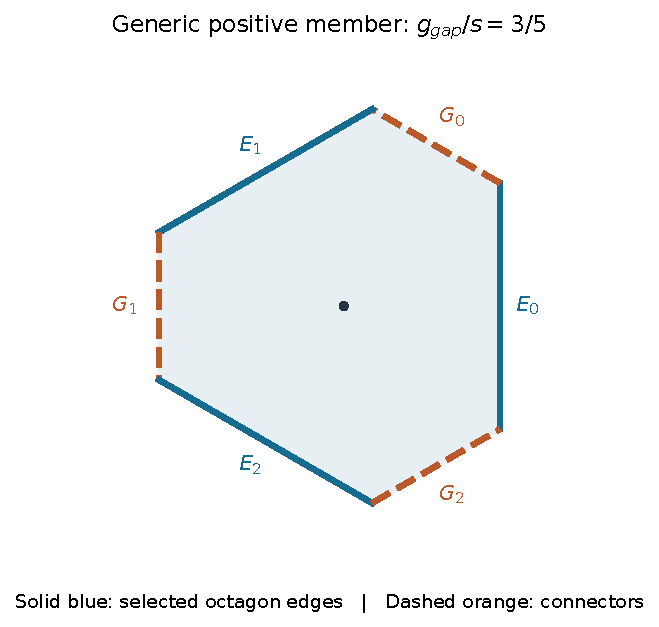
\includegraphics[width=0.78\linewidth,height=\textheight,keepaspectratio,alt={A generic member with g\_\{\textbackslash mathrm\{gap\}\}/s=3/5. Solid edges are selected octagon edges; dashed edges are deliberate connectors. The lengths alternate while every turn remains 60\^{}\textbackslash circ.}]{figures/03_alternating.pdf}
\caption{A generic member with \(g_{\mathrm{gap}}/s=3/5\). Solid edges are selected octagon edges; dashed edges are deliberate connectors. The lengths alternate while every turn remains \(60^\circ\).}
\end{figure}

The gap subscript will be retained even in the geometric sections. The recurrence coefficient historically written \texttt{g} is denoted \(g_{\mathrm{coupling}}\) in Section 16. It is a parameter of a state update, not a reference length, and no equation in this paper identifies the two.

\section{7. Exact regularity theorem}\label{exact-regularity-theorem}

\textbf{Theorem 2 (alternating hexagon and regularity).} Let \(s>0\) and \(g_{\mathrm{gap}}>0\), set \(p\) by (8), and form (5). The chain is the boundary of a convex hexagon. It has alternating side lengths \(s,g_{\mathrm{gap}}\), every exterior turn is \(+60^\circ\), and every interior angle is \(120^\circ\). It is regular if and only if

\paperdisplay[9]{g_{\mathrm{gap}}=s
\quad\Longleftrightarrow\quad
p=p_*:=\frac{\sqrt3}{2}s.}

\textbf{Proof.} Write \(d_k=H_{k+1}-H_k\), with indices modulo six, and let \(\ell_k\) alternate between \(s\) and \(g_{\mathrm{gap}}\). Lemma 1 gives successive unit directions \(t_0,R_{60}t_0,t_1,R_{60}t_1,t_2,R_{60}t_2\). Since \(t_{i+1}=R_{120}t_i\), each direction is the counterclockwise \(60^\circ\) rotation of the preceding one. Therefore

\paperdisplay[10]{\begin{gathered}
|d_k|=\ell_k,\qquad
d_{k-1}\cdot d_k=\tfrac12\ell_{k-1}\ell_k,\\
\det(d_{k-1},d_k)=\tfrac{\sqrt3}{2}s g_{\mathrm{gap}}>0,
\qquad \sum_{k=0}^{5}d_k=0.
\end{gathered}}

The final identity follows by telescoping the closed endpoint list; equivalently, each of the two three-vector direction orbits sums to zero. The positive determinants fix orientation and exclude straight or reversed consecutive edges. The interior-angle cosine is \((-d_{k-1})\cdot d_k/(\ell_{k-1}\ell_k)=-1/2\).

A local turn computation alone should not be substituted for a global simplicity argument. The independent support-triangle construction in Proposition 4 below shows that this exact chain bounds the intersection of an equilateral triangle with three inward corner-cut half-planes. The residual side length is \(s>0\), and every connector has positive length. That intersection is convex and has precisely these six edges. Thus the computed angles are the polygon\textquotesingle s interior angles.

A regular polygon must have equal sides, so regularity forces \(g_{\mathrm{gap}}=s\). Conversely, at that equality, all six sides and all six angles are equal. It is therefore a regular hexagon. Substitution into (8) gives the equivalent midpoint radius in (9). \(\square\)

\begin{figure}
\centering
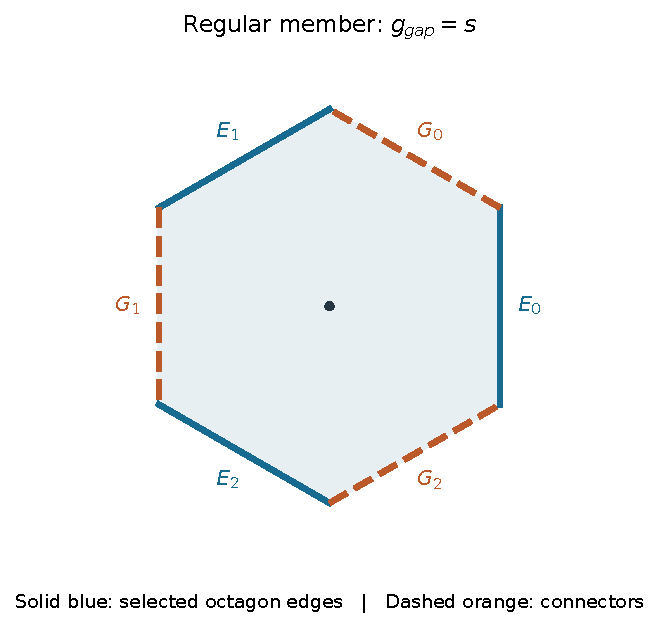
\includegraphics[width=0.78\linewidth,height=\textheight,keepaspectratio,alt={The regular case, with roles retained. Although all six side lengths are equal, the blue and orange edge classes record different construction origins.}]{figures/04_regular_roles.pdf}
\caption{The regular case, with roles retained. Although all six side lengths are equal, the blue and orange edge classes record different construction origins.}
\end{figure}

The theorem is an exact statement about the aligned family, not a numerical observation and not a theorem that arbitrary three octagons produce a regular core. Alignment, ordering, positivity and tuning each have a separate role in the proof. Removing any of those hypotheses requires a different statement.

\section{8. Explicit vertices and metric consequences}\label{explicit-vertices-and-metric-consequences}

Substituting (8) into (4) gives the following complete coordinate prescription:

\paperdisplay[11]{\begin{aligned}
H_0&=(p,-s/2), & H_1&=(p,s/2),\\
H_2&=\left(\frac{s-g_{\mathrm{gap}}}{2\sqrt3},\frac{s+g_{\mathrm{gap}}}{2}\right),&
H_3&=\left(-\frac{2s+g_{\mathrm{gap}}}{2\sqrt3},\frac{g_{\mathrm{gap}}}{2}\right),\\
H_4&=\left(-\frac{2s+g_{\mathrm{gap}}}{2\sqrt3},-\frac{g_{\mathrm{gap}}}{2}\right),&
H_5&=\left(\frac{s-g_{\mathrm{gap}}}{2\sqrt3},-\frac{s+g_{\mathrm{gap}}}{2}\right).
\end{aligned}}

\textbf{Proposition 3 (radii and area).} The six vertices lie on the circle centred at the origin with radius \(R_H\), and the polygon has area \(\mathcal A_H\), where

\paperdisplay[12]{R_H^2=\frac{s^2+s g_{\mathrm{gap}}+g_{\mathrm{gap}}^2}{3},\qquad
\mathcal A_H=\frac{\sqrt3}{4}
\left(s^2+4s g_{\mathrm{gap}}+g_{\mathrm{gap}}^2\right).}

\textbf{Proof.} Each endpoint has squared norm \(p^2+s^2/4\) because \(u_i\) and \(t_i\) are orthonormal. Inserting (8) gives the radius formula. Proposition 4 partitions the support triangle into this hexagon and three equilateral triangles of side \(g_{\mathrm{gap}}\). Their areas subtract to

\paperdisplay[]{\frac{\sqrt3}{4}\left((s+2g_{\mathrm{gap}})^2-3g_{\mathrm{gap}}^2\right),}

which expands to the second expression. These arguments prove the identities for arbitrary positive lengths. \(\square\)

The distances from the origin to the selected-edge lines and connector lines are respectively

\paperdisplay[13]{p=\frac{s+2g_{\mathrm{gap}}}{2\sqrt3},\qquad
q_H=\frac{2s+g_{\mathrm{gap}}}{2\sqrt3}.}

For example, the unit outward normal to \(G_0\) is \(R_{60}u_0\). Its dot product with \(B_0\) is \(p/2+\sqrt3s/4=q_H\). By cyclic symmetry this holds at all connectors. Thus the generic polygon is cyclic but does not have one origin-centred circle tangent to all six sides. A common incircle, if present, must have a centre fixed by the threefold symmetry: uniqueness follows already from equal distances to the three selected-edge support lines. It therefore exists exactly when \(p=q_H\), which is \(s=g_{\mathrm{gap}}\).

In the regular case (11) reduces to

\paperdisplay[14]{H_k=s\bigl(\cos(-\pi/6+k\pi/3),\sin(-\pi/6+k\pi/3)\bigr),
\qquad k=0,\ldots,5.}

These are standard regular-hexagon coordinates rotated by \(-30^\circ\); a common translation places their centre anywhere desired. The side length and circumradius both equal \(s\), the inradius is \(\sqrt3s/2\), the perimeter is \(6s\), and the area is \(3\sqrt3s^2/2\). Euclid\textquotesingle s construction of a regular hexagon and its radius-side corollary provide a classical reference {[}R1{]}. Here (14) supplies the direct coordinate verification needed for the model.

\section{9. Support triangle and the three reference gap cells}\label{support-triangle-and-the-three-reference-gap-cells}

The support triangle explains the geometry without requiring visible octagons. Let

\paperdisplay[15]{\mathcal T=\{x\in\mathbb R^2:u_i\cdot x\le p\text{ for }i=0,1,2\},
\qquad V_i=p u_i+\sqrt3p\,t_i.}

The point \(V_i\) lies on the support lines for \(i\) and \(i+1\). For instance, \(V_0=(p,\sqrt3p)\) satisfies both \(x=p\) and \(-x/2+\sqrt3y/2=p\). The third support inequality is strict there. Rotation generates the other vertices.

\textbf{Proposition 4 (equilateral truncation).} The set \(\mathcal T\) is an equilateral triangle of side

\paperdisplay[16]{W=2\sqrt3p=s+2g_{\mathrm{gap}}.}

For each \(i\), the closed corner cell \(\operatorname{conv}\{B_i,V_i,A_{i+1}\}\) is equilateral of side \(g_{\mathrm{gap}}\). With \(n_i^G=R_{60}u_i\) and \(q_H=(2s+g_{\mathrm{gap}})/(2\sqrt3)\), the closed filled residual hexagon is precisely

\paperdisplay[16a]{\mathcal H=\mathcal T\cap\bigcap_{i=0}^{2}
\{x\in\mathbb R^2:n_i^G\cdot x\le q_H\}.}

Its ordered vertices are (11). Equivalently, remove \(\mathcal T\cap\{x:n_i^G\cdot x>q_H\}\) at each corner, retaining the connector as boundary. Removing only the ordinary two-dimensional open interior of a corner cell would incorrectly leave its apex and outer legs. For example,

\paperdisplay[16b]{n_0^G\cdot V_0-q_H=\frac{\sqrt3}{2}g_{\mathrm{gap}}>0,}

so \(V_0\) is outside \(\mathcal H\) even though it is not in that cell\textquotesingle s open interior. The closed half-plane definition removes this boundary ambiguity without changing the lengths or area.

\textbf{Proof.} On support line \(i\), the two adjacent support vertices occur at local tangent coordinates \(-\sqrt3p\) and \(+\sqrt3p\). Their distance is \(2\sqrt3p\). Rotation makes all three sides equal. The support-line normals differ by \(120^\circ\), so the triangle\textquotesingle s interior angles are \(60^\circ\).

The distance from \(B_i\), whose tangent coordinate is \(s/2\), to \(V_i\) is \(\sqrt3p-s/2=g_{\mathrm{gap}}\). The analogous distance from \(V_i\) to \(A_{i+1}\) on the next side is the same. Lemma 1 gives the third side of the corner triangle as \(g_{\mathrm{gap}}\). It is therefore equilateral. Along each support side, the two removed corner legs consume \(2g_{\mathrm{gap}}\) of its length \(W\) and leave exactly \(s>0\) between them.

For a global nonoverlap argument, use barycentric coordinates of \(\mathcal T\). Each corner triangle consists of points whose barycentric coordinate at that corner is at least \(1-g_{\mathrm{gap}}/W\). Since \(2g_{\mathrm{gap}}<W\), this threshold exceeds \(1/2\). Two distinct corner interiors cannot both contain a point, because its barycentric coordinates sum to one. The three cutting half-planes therefore leave a convex polygon with six positive edges, exactly the endpoint and connector list already specified. This also completes the convexity argument in Theorem 2. \(\square\)

\begin{figure}
\centering
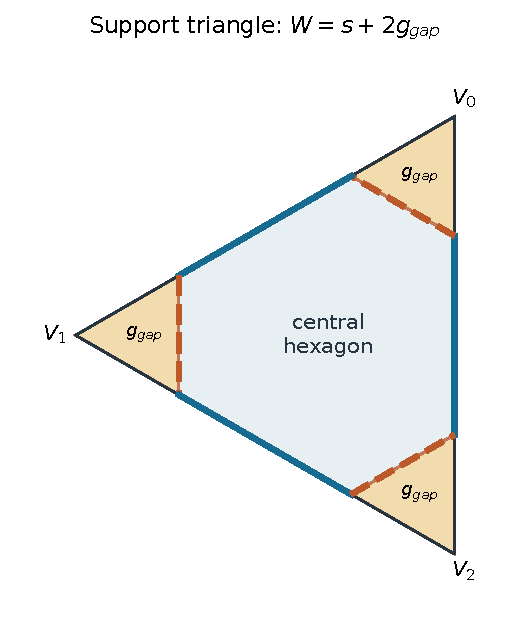
\includegraphics[width=0.81\linewidth,height=\textheight,keepaspectratio,alt={The equilateral support triangle and its three corner cells for g\_\{\textbackslash mathrm\{gap\}\}/s=3/5. Each support side divides into lengths g\_\{\textbackslash mathrm\{gap\}\},s,g\_\{\textbackslash mathrm\{gap\}\}. The central region has the six vertices in (11).}]{figures/05_support_triangle.pdf}
\caption{The equilateral support triangle and its three corner cells for \(g_{\mathrm{gap}}/s=3/5\). Each support side divides into lengths \(g_{\mathrm{gap}},s,g_{\mathrm{gap}}\). The central region has the six vertices in (11).}
\end{figure}

The word gap here names a reference cell in a construction. The cells have exact locations and boundaries; this is more information than an unspecified angular window. But the construction does not assert that each is a complete component of physical empty space, a triangular material face or a region with a prescribed field. A field domain would require additional choices concerning interiors, boundaries and coupling to neighboring objects.

At regularity, \(W=3s\). The support triangle divides into three equilateral corner triangles of side \(s\) and one central regular hexagon of side \(s\). This is a standard Euclidean construction that can be performed with a straightedge and compass. In particular, trisect each side by equal-length marks and connect adjacent marks around each corner. No E8 projection, dynamical trajectory or numerical optimization is needed.

\begin{figure}
\centering
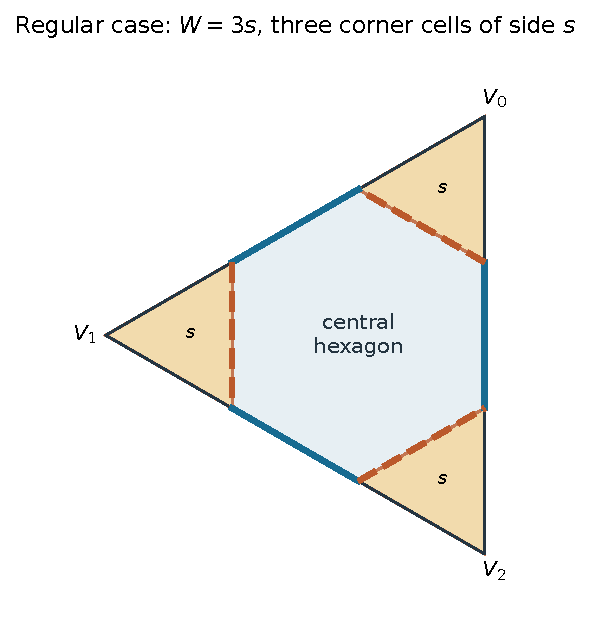
\includegraphics[width=0.81\linewidth,height=\textheight,keepaspectratio,alt={At regularity, an equilateral triangle of side 3s loses three equilateral corner triangles of side s. The retained central hexagon has six equal sides and 120\^{}\textbackslash circ interior angles.}]{figures/06_regular_truncation.pdf}
\caption{At regularity, an equilateral triangle of side \(3s\) loses three equilateral corner triangles of side \(s\). The retained central hexagon has six equal sides and \(120^\circ\) interior angles.}
\end{figure}

The total triangle area is \(9\sqrt3s^2/4\); the corner area is \(3\sqrt3s^2/4\); their difference is \(3\sqrt3s^2/2\). This checks the regular specialization of (12) by an independent dissection. The support triangle is consequently both a proof device and a compact replacement for a display of all three octagons.

\section{10. Symmetry of unmarked and role-marked objects}\label{symmetry-of-unmarked-and-role-marked-objects}

We use \(C_n\) for rotations of order \(n\) and \(D_n\) for the dihedral group of order \(2n\). Stating the convention avoids the conflicting uses of labels such as D24 in historical material. Three objects must be distinguished: the unmarked polygon, the polygon with its E/G edge classes retained, and the complete collection of octagonal reference figures.

\textbf{Proposition 5 (symmetry and role exchange).} For \(s\ne g_{\mathrm{gap}}\), the unmarked hexagon has symmetry group \(D_3\). At \(s=g_{\mathrm{gap}}\), that group enlarges to \(D_6\). Preserving the E/G classes restricts the regular polygon back to \(D_3\).

\textbf{Proof.} Rotation by \(120^\circ\) preserves (4). Reflection across the \(u_0\) axis swaps \(A_0\) with \(B_0\) and interchanges the other selected edges. It also permutes the connectors. These operations generate \(D_3\). In a convex hexagon, an isometry induces an adjacency-preserving permutation of vertices, hence an element of the abstract dihedral group of a six-cycle. If the two alternating lengths differ, an odd edge shift cannot preserve lengths. Only the even rotations and the three corresponding reflections survive, so there are no extra symmetries beyond \(D_3\).

At equality, (14) exhibits all rotations through multiples of \(60^\circ\) and all six reflection axes, giving \(D_6\). A \(60^\circ\) rotation advances the cyclic edge list by one place and exchanges E and G. If those roles must be preserved, only the previous subgroup remains. \(\square\)

This claim concerns role classes, not three immovable letter labels. It allows simultaneous permutation of the three indexed frames. Requiring each label to remain pointwise fixed would be a different marking problem. Requiring the traversal orientation to be preserved also excludes the reflections, leaving the rotational subgroup \(C_3\) of the role-marked object.

The explicit complete-frame construction in Section 11 has \(D_3\) symmetry for the same covariant placement. Its three noncollinear frame centres form an equilateral triangle, whose symmetry group supplies an upper bound when individual frames are retained as constituents. Thus the extra unmarked hexagon symmetry does not become a symmetry of the full three-frame construction. Forgetting reference roles changes the object whose symmetry is being measured.

\section{11. Completing the regular octagon reference frames}\label{completing-the-regular-octagon-reference-frames}

The construction has so far used three selected segments. It remains to show that these really can belong to complete regular octagons with the prescribed common side length. The filled reference region in (2a) supplies an explicit completion:

\paperdisplay[17]{C_i=(p+a)u_i,\qquad
\mathcal O_i=\{C_i+xu_i+yt_i:(x,y)\in\mathcal O_s\}.}

Each map from the local plane is an orientation-preserving isometry. Applied to \(\mathcal O_s\), it gives the filled reference region \(\mathcal O_i\) in (17); applied to \(\partial\mathcal O_s\) or the ordered vertices \(\mathcal V_s\), it gives the outline or ordered vertex list. Its inward side has local \(x=-a\) and \(y\in[-s/2,s/2]\), so its global coordinates are \(p u_i+y t_i\). Its endpoints are precisely \(A_i,B_i\).

\textbf{Proposition 6 (complete-frame existence).} Equations (2) and (17) realize the selected edges in three complete regular octagonal reference figures. At regularity their centre radius is

\paperdisplay[18]{L_*=a+p_* =\frac{1+\sqrt2+\sqrt3}{2}s.}

\textbf{Proof.} The isometry argument proves regularity and side length, the inward-side calculation proves endpoint agreement, and substitution of (1) and (9) proves (18). \(\square\)

\begin{figure}
\centering
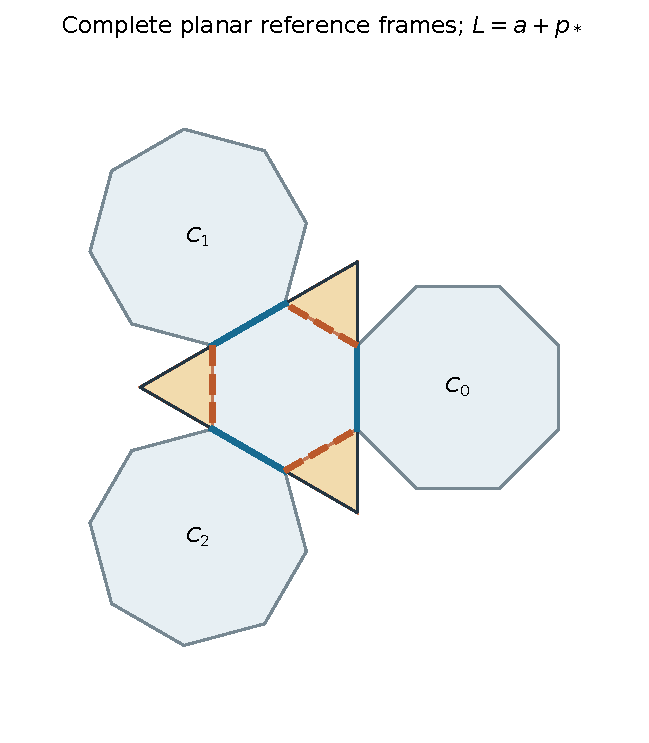
\includegraphics[width=0.9\linewidth,height=\textheight,keepaspectratio,alt={Complete planar reference figures at regularity. The inward sides generate the blue edge class; orange connectors close the central chain. The three corner cells remain visible without treating them as physical material or holes in a welded mesh.}]{figures/07_complete_frames.pdf}
\caption{Complete planar reference figures at regularity. The inward sides generate the blue edge class; orange connectors close the central chain. The three corner cells remain visible without treating them as physical material or holes in a welded mesh.}
\end{figure}

The midpoint radius \(p\) is not the planar octagon centre radius \(L=p+a\). Interchanging them would produce a different connector length. The distinction also explains why a later shrink rule for vertical face centres cannot be applied unchanged to these planar centres.

This realization proves existence, not uniqueness. A selected edge can support other placements of a complete reference figure, including three-dimensional embeddings. Only one convenient covariant planar completion is required to establish that the scaffold is compatible with full octagons. No collision-free deployment motion, unique historical placement or tiling claim follows.

The octagons lie on the outward sides of their inward selected-edge support lines. The central support triangle is on the inward side of all three. Thus its interior and the displayed corner-cell interiors are outside the interiors of these particular planar octagons. That property clarifies the drawing but is not used to demand that the hexagon boundary be made entirely of octagon sides: half its sides remain deliberate connectors.

\section{12. The vertical-face family and the exact Paper-C comparison}\label{the-vertical-face-family-and-the-exact-paper-c-comparison}

A different embedding maps the filled local region \(\mathcal O_s\) in (2a) into a vertical plane. To avoid confusing a scalar local coordinate with the vector \(u_i\), write the former as \(\xi\):

\paperdisplay[19]{F_i(\xi,z)=p u_i+\xi t_i+z e_z,
\qquad (\xi,z)\in\mathcal O_s.}

The notation embeds the two-dimensional \(u_i,t_i\) into the horizontal plane. The finite filled face is \(F_i(\mathcal O_s)\); its outline is \(F_i(\partial\mathcal O_s)\) and its eight vertices are the images of \(\mathcal V_s\). Here the vertical face centre is \(p u_i\), so its centre radius is \(p\), unlike the planar centre radius \(L\) in (17). The top edge is at \(z=a\) and \(\xi\in[-s/2,s/2]\). Its horizontal coordinates again equal (4). The six top endpoints therefore determine the same measurement-polygon family.

\textbf{Proposition 7 (Paper-C measurement member).} Set \(p_0=a/\sqrt3\). Applying the rigid map

\paperdisplay[20]{M(x)=R_z(\pi/6)x+(0,a/\sqrt3,0)}

to the three faces (19) gives the Paper-C panels in the order \(i=0,1,2\mapsto P_3,P_1,P_2\), where

\paperdisplay[21]{\begin{aligned}
P_1(\xi,z)&=(-a/2-\xi/2,\sqrt3a/2-\sqrt3\xi/2,z),\\
P_2(\xi,z)&=(\xi,0,z),\\
P_3(\xi,z)&=(a/2-\xi/2,\sqrt3a/2+\sqrt3\xi/2,z).
\end{aligned}}

Its top measurement polygon satisfies

\paperdisplay[22]{p_0=\frac{(1+\sqrt2)s}{2\sqrt3},\qquad
g_{\mathrm{gap},0}=\sqrt3p_0-s/2=\frac{s}{\sqrt2}.}

\textbf{Proof.} Insert the three frames (3) into (19), rotate by \(30^\circ\) and add the translation. For \(i=0\), the horizontal coordinates become \((\sqrt3p_0/2-\xi/2,p_0/2+\sqrt3\xi/2+a/\sqrt3)\), which reduce to \(P_3\). The other two substitutions give \(P_1,P_2\). Since the same local octagon domain is used, this is an identity of finite faces, not merely of supporting planes. Equation (22) follows from (1) and (8). \(\square\)

\begin{figure}
\centering
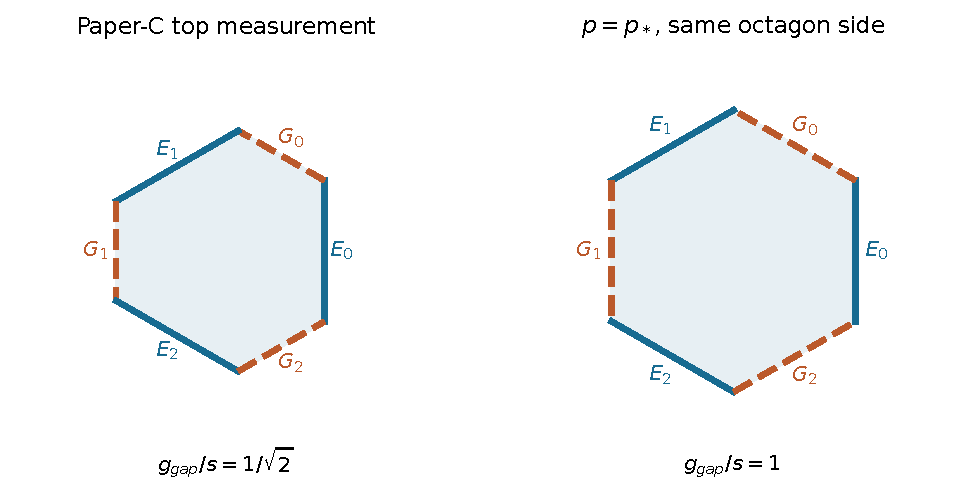
\includegraphics[width=0.98\linewidth,height=\textheight,keepaspectratio,alt={Paper C\textquotesingle s top measurement polygon and the regular reference member at the same selected-edge length. The six top points belong to one aligned family, while the two placements have different finite-face incidence.}]{figures/08_paper_c_measurement.pdf}
\caption{Paper C\textquotesingle s top measurement polygon and the regular reference member at the same selected-edge length. The six top points belong to one aligned family, while the two placements have different finite-face incidence.}
\end{figure}

Paper C therefore has six top measurement lengths alternating between \(s\) and \(s/\sqrt2\), with all six angles equal to \(120^\circ\). The connector chords partition a measurement polygon; they are not additional edges of the welded mesh. Its actual nonplanar rim has nine edges. Equating that rim with the six-point polygon would erase part of the finite surface.

The rigid identity proves a precise relation between two specified coordinate descriptions. It does not identify the full Paper-C shell with every historical Tri-Octagon construction, prove that Paper C was intended to have a regular top hexagon, or make its published unequal-length result an error. The distinction between the measurement family and surface incidence is what permits an exact comparison without rewriting either object.

\section{13. Two different tuning operations}\label{two-different-tuning-operations}

The regularity condition can be reached in two ways within the vertical-face family. Each changes a different parameter and has a different spatial consequence. Both should be distinguished from a common similarity applied to the whole arrangement.

\subsection{13.1 Fixed size, outward translation}\label{fixed-size-outward-translation}

Keep \(s,a\) and each face orientation fixed. Change the midpoint/face-centre radius from \(p_0\) to \(p_*\). The required displacement of face \(i\) is \(\Delta p\,u_i\), with

\paperdisplay[23]{\Delta p=p_*-p_0=\frac{(2-\sqrt2)s}{2\sqrt3}>0,
\qquad \frac{p_*}{p_0}=\frac{3}{1+\sqrt2}.}

This follows by subtracting (22) from (9). The top height remains \(a\) because the motion is horizontal. The selected-edge length remains \(s\), while the connector length increases to \(s\). Equation (23) is a placement operation, not a rule for the state recurrence.

\subsection{13.2 Fixed vertical face centres, individual shrink}\label{fixed-vertical-face-centres-individual-shrink}

Instead keep each face centre \(p_0u_i\) fixed and multiply all local coordinates \((\xi,z)\) by a positive factor \(\lambda\). The new side and apothem are \(s'=\lambda s\) and \(a'=\lambda a\). The midpoint radius remains \(p_0\), while the selected top plane moves from \(z=a\) to \(z=a'\).

Imposing regularity on the new top chain requires

\paperdisplay[]{\sqrt3p_0-\frac{\lambda s}{2}=\lambda s.}

Using \(\sqrt3p_0=a=(1+\sqrt2)s/2\) gives the unique positive solution

\paperdisplay[24]{\lambda=\frac{1+\sqrt2}{3}\simeq0.804737854,
\qquad s'=g'_{\mathrm{gap}}=\lambda s.}

The word fixed refers to the three vertical face centres, not to the original top endpoints or top height. The latter change. Shrinking about the planar centres \(C_i\) in (17) is another operation: then the selected-edge midpoint radius is \(L-\lambda a\), rather than the fixed \(p_0\) assumed above. Formula (24) must not be transferred to that operation without a new derivation.

\subsection{13.3 Why a global scale change does not tune the shape}\label{why-a-global-scale-change-does-not-tune-the-shape}

Under a common similarity with scale factor \(c>0\), both \(p\) and \(s\) become \(cp,cs\). Equation (8) then gives \(g_{\mathrm{gap}}\mapsto c g_{\mathrm{gap}}\), leaving \(g_{\mathrm{gap}}/s\) unchanged. A width change caused by rescaling the entire arrangement does not turn \(1/\sqrt2\) into one.

An invertible affine transformation preserves collinearity, incidence, parallelism and ratios along a line. It need not preserve angles or equal lengths in different directions. Thus its image of the triangular truncation still has corresponding incidence, but need not be a regular hexagon. The tuning and metric statements here use Euclidean similarities, not arbitrary affine invariance of regularity.

\section{14. Width-one shrink and finite-face consequences}\label{width-one-shrink-and-finite-face-consequences}

\subsection{14.1 Exact worked example}\label{exact-worked-example}

Start from Paper C\textquotesingle s width-one normalization:

\paperdisplay[25]{w_0=1,\qquad a_0=\frac12,\qquad s_0=\sqrt2-1,
\qquad p_0=\frac1{2\sqrt3}.}

At fixed centres, (24) gives

\paperdisplay[26]{s'=\frac{(1+\sqrt2)(\sqrt2-1)}3=\frac13,
\qquad g'_{\mathrm{gap}}=\sqrt3p_0-\frac{s'}2=\frac13.}

All six resulting sides are therefore exactly \(1/3\). The product in (26) is exactly one before division, not an approximate cancellation. The support side stays \(W=2\sqrt3p_0=1\). The final hexagon has circumradius \(1/3\), inradius \(\sqrt3/6\) and area \(\sqrt3/6\).

The octagons themselves no longer have width one:

\paperdisplay[27]{w'=\frac{1+\sqrt2}{3},\qquad
z'_{\mathrm{top}}=a'=\frac{1+\sqrt2}{6}<\frac12.}

The lowered top plane is part of the actual three-dimensional shrink. A figure that shows only outward translation at height \(1/2\) cannot illustrate this operation.

\begin{figure}
\centering
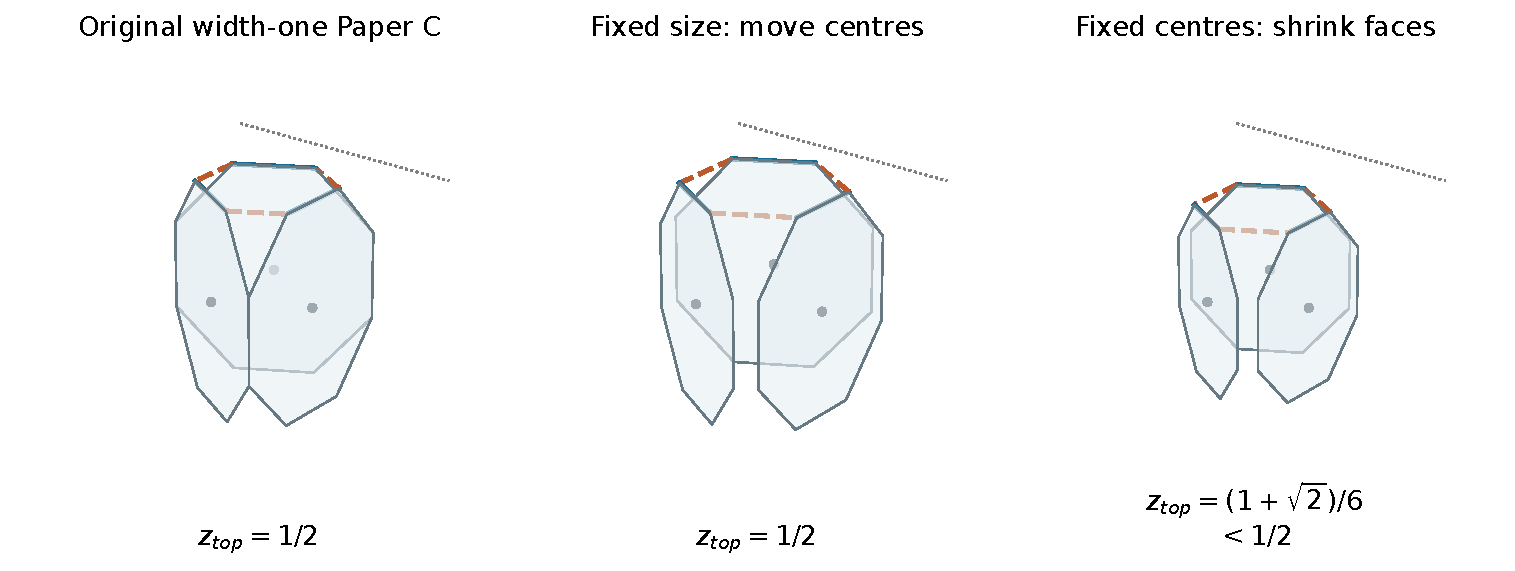
\includegraphics[width=1\linewidth,height=\textheight,keepaspectratio,alt={Equal-scale views of the width-one starting module, fixed-size outward translation and fixed-centre shrink. Black points mark face centres. The dotted height reference is the original z=1/2; shrinking lowers the top to (1+\textbackslash sqrt2)/6. Top connectors are construction lines, not new material strips.}]{figures/09_translation_and_shrink.pdf}
\caption{Equal-scale views of the width-one starting module, fixed-size outward translation and fixed-centre shrink. Black points mark face centres. The dotted height reference is the original \(z=1/2\); shrinking lowers the top to \((1+\sqrt2)/6\). Top connectors are construction lines, not new material strips.}
\end{figure}

\subsection{14.2 Supporting planes versus finite faces}\label{supporting-planes-versus-finite-faces}

\textbf{Proposition 8 (seam loss and separation).} For the finite filled faces \(F_i(\mathcal O_s)\) defined in (19), adjacent supporting planes intersect at local coordinates \(\xi=+\sqrt3p\) and \(\xi=-\sqrt3p\). At \(p=p_0=a/\sqrt3\) the finite faces share a full side seam. For \(p>p_0\) they are disjoint, with minimum Euclidean separation

\paperdisplay[28]{\delta_{\mathrm{face}}=\sqrt3p-a.}

\textbf{Proof.} Solve the two horizontal supporting-line equations from (19); the local tangent coordinates have the stated opposite signs. A finite octagon obeys \(|\xi|\le a\). At equality \(\xi=\pm a\), its vertical side runs over \(z\in[-s/2,s/2]\), yielding the Paper-C seam. When \(\sqrt3p>a\), the line intersection lies beyond both finite faces, although the infinite planes continue to intersect.

For a distance bound, take points on the two faces with local coordinates \(\xi=a-X\) and \(\eta=-a+Y\), where \(X,Y\ge0\). Direct expansion of (19) yields

\paperdisplay[29]{\begin{aligned}
|F_i(\xi,z)-F_{i+1}(\eta,z')|^2
={}&\delta_{\mathrm{face}}^2+\delta_{\mathrm{face}}(X+Y)\\
&+(X-Y)^2+XY+(z-z')^2.
\end{aligned}}

Every term beyond \(\delta_{\mathrm{face}}^2\) is nonnegative for \(p\ge p_0\). Equality is attained at \(X=Y=0\) and a common height on the side intervals. This proves (28), including its sharpness. The threefold symmetry covers every pair. \(\square\)

At the translated regular member, the separation is \((2-\sqrt2)s/2>0\). At the fixed-centre shrink of (25), it is \(a_0-a'=(2-\sqrt2)/6>0\). Both operations therefore destroy the original seams. The original mesh has 18 distinct vertices, 21 edges and three faces, forming an annulus with two nine-edge boundary cycles. The separated realization contains 24 vertices, 24 edges and three disjoint octagonal disks, with three eight-edge boundaries, when only the original faces are counted. These are established finite-mesh counts in {[}I2,I5{]}, not a new mesh generation here.

Adding reference connectors does not glue the faces or supply new two-dimensional faces. The regular measurement polygon consequently coexists with disconnected finite panels. Within this particular fixed-orientation family, original welding and the regular condition cannot both hold for unchanged regular octagons. This is a scoped geometric consequence, not a universal obstruction to other reference constructions.

\section{15. What the octagons determine}\label{what-the-octagons-determine}

The octagons determine a reproducible selected-edge length and orientation, a scale through their width or apothem, three covariant reference frames, and the endpoints used in the connector construction. Through those endpoints they determine the support triangle, its corner cells and the derived polygon. These are real mathematical constraints: changing the alignment or the spacing changes the construction.

They need not be physical matter, tile a plane, remain visible in a final display, or form a connected surface. Neither filling the polygons nor removing their outlines changes a previously defined endpoint formula. A downstream object can retain an incidence relation generated by reference figures that are absent from its final rendering.

This makes the reference scaffold different from a material mesh without making every associated calculation merely illustrative. If a function consults scaffold coordinates and changes a later state, that is an implemented geometric coupling. If it maps a state to display coordinates without returning them to the state, it is a readout or display map. If no such function is specified, the interface is open. The following section applies that operational distinction to surviving historical code.

The earlier filled-planar-hole obstruction remains valid under its original stronger hypotheses. For an interior-disjoint arrangement of filled regular octagons with a regular hexagonal hole bounded entirely by actual octagon sides, a \(120^\circ\) hole corner leaves only \(240^\circ\) outside the hole. One convex octagon cannot provide the hole\textquotesingle s concave complement; two incident octagon corners require at least \(135^\circ+135^\circ=270^\circ\) without interior overlap. A corner in the interior of an octagon side consumes still more. Under the stated incidence hypotheses this is impossible {[}I2, Section 2{]}.

That argument does not concern the present chain: three of its sides are connectors, and it is not required to be a hole bounded entirely by material octagon edges. Keeping a correct obstruction attached to its hypotheses prevents both rejecting the intended scaffold and weakening the original theorem.

\section{16. Relation to toy-model functionality: established links and open interfaces}\label{relation-to-toy-model-functionality-established-links-and-open-interfaces}

\subsection{16.1 The clarified recollection and the bounded question}\label{the-clarified-recollection-and-the-bounded-question}

The author tentatively associated the recollection with a Z-vector or torus display. This guided the bounded source trace; it did not identify the exact historical implementation or its registration with the gap geometry. The existing response record contains an explicit adopted relay of assisted wording. That adoption is distinct from an independently recalled or source-verified mechanism, and does not by itself exclude other historical candidates or raise their source-evidence confidence.

The following account is a static trace of functions already identified in the existing source map {[}I6{]}. No historical system was launched, repaired or fitted. Source versions and function anchors are bound in the package\textquotesingle s provenance manifest. The exact conclusion is that several Z/readout-to-display maps survive, while their coordinate registration with the triangular cells of Section 9 is absent from the inspected functions.

\subsection{16.2 The historical triad and its readouts}\label{the-historical-triad-and-its-readouts}

The staged \texttt{model\_core.py} evolves \(\Omega\in\mathbb C^3\). Its unforced pre-synchronization update has the form

\paperdisplay[30]{V=\Omega+\varepsilon\Omega\odot(k-|\Omega|^2)
+g_{\mathrm{coupling}}L_3\Omega,\qquad
(L_3)_{ii}=-2,\quad (L_3)_{ij}=1\ (i\ne j).}

An optional offset, simultaneous third-harmonic phase correction and optional noise are separate operations in that source. Typical defaults are \(\varepsilon=.05\), \(g_{\mathrm{coupling}}=.2\) and phase coefficient \(.001\). With the default clock setting, a mod-12 external counter \(q\) and scalar time advance alongside the state. The argument \texttt{dt} advances that scalar time; it does not multiply the increment in (30).

Writing \(\vartheta=2\pi q/12\), \(\kappa=\|\Omega\|\) and \(\rho=\kappa/(1+\kappa)\), the working readout variant computes

\paperdisplay[31]{z=.618\rho\cos(3(\vartheta-.244))e^{-.577t},\qquad
Z_{\mathrm{macro}}=z(\cos\vartheta,\sin\vartheta,1),}
\paperdisplay[32]{\begin{aligned}
Z_{\mathrm{chiral}}&=(\Im\bar\Omega_2\Omega_3,
\Im\bar\Omega_3\Omega_1,\Im\bar\Omega_1\Omega_2),\\
Z_{\mathrm{total}}&=Z_{\mathrm{macro}}+.5Z_{\mathrm{chiral}}.
\end{aligned}}

The decimal coefficients in (31) are literal source values; no exact-constant repair is made here. The vector \(Z_{\mathrm{chiral}}\) is bilinear and depends on amplitudes as well as phases. It \textbf{has no imposed decay envelope; need not decay}. These are channel observables; an explicit map is needed to use them as spatial display coordinates. Such a display assignment alone does not establish a physical position or energy.

The captured historical committed core has a different scalar law. With \(J=\Im(\Omega_1\bar\Omega_2\Omega_3)\), it updates \(m^+=.99m+.01J/(1+|J|)\) and uses \(z=.618\rho\cos(3(\vartheta-.244))+m^+\), without the exponential envelope. Both versions feed these readouts to records and consumers rather than back into later \(\Omega\) at fixed supplied parameters. A history sample is recorded before the next step, and initial stored readouts are zero. These temporal details matter when interpreting a saved curve.

\subsection{16.3 Three source-supported display candidates}\label{three-source-supported-display-candidates}

\textbf{Z-vector overlay.} The function \texttt{history\_Zvec\_to\_xyz} in \texttt{geometry\_3d.py} returns stored vector components, normally \texttt{Z\_total}, with a legacy \texttt{Z\_vec} fallback. In \texttt{toy\_3d\_triocta.py}, \texttt{\_get\_Z\_scaled} divides by the 99th percentile of finite vector norms exceeding \(10^{-12}\), with denominator fallback one, and multiplies by \(.85r_{\mathrm{frame}}\), where \(r_{\mathrm{frame}}=.6\). The plotting consumer draws the resulting curve, and a selector chooses total, macro, chiral or off. This is a specific surviving Z geometry compatible with the author\textquotesingle s tentative Z/torus association. The whole-history scale is a display normalization; it is not an amplitude update.

\textbf{Clock/scalar torus map.} The function \texttt{history\_to\_torus\_xyz} instead uses the recorded norm, clock and scalar \(z\). Its exact form is

\paperdisplay[33]{\begin{gathered}
r=r_{\max}\frac{\kappa}{1+\kappa},\quad
\varphi=\frac{2\pi q}{12},\quad
\chi=\frac{\pi}{2}\frac{z}{\max_{\mathrm{history}}|z|+10^{-9}},\\
T=((R+r\cos\chi)\cos\varphi,
(R+r\cos\chi)\sin\varphi,r\sin\chi),
\end{gathered}}

with defaults \(R=2,r_{\max}=1\). The consumer \texttt{plot\_torus\_trajectory\_3d} in \texttt{analysis\_tools.py} plots these arrays. Its effective import is the \texttt{geometry\_3d} version, which shadows an earlier same-named import. A second function gives cylindrical coordinates \((\kappa\cos\varphi,\kappa\sin\varphi,z)\). These are distinct readout maps. The retrospective denominator in (33) also prevents interpreting the displayed coordinate as an autonomous causal state variable.

\textbf{Channel-phase torus map.} The viewer\textquotesingle s \texttt{embed\_on\_torus} uses each channel directly. It fixes azimuth \(\alpha_j=2\pi j/3\), takes minor angle \(\arg\Omega_j\), and chooses tube radius \(.6(1+.4\log(1+|\Omega_j|))\). Inserting those quantities into the torus coordinate form produces three channel curves. This map uses neither the scalar \(z\) nor the mod-12 clock in (33). Its diagnostic corridor function separately bins \(\arg(\operatorname{mean}\Omega)\) into 12 sectors; it does not recover the external counter by identity.

These maps are established source-to-display links. Identification of one as the exact remembered gap-related scene remains a plausible lead. None of the inspected function bodies consumes the endpoints (4), the corner triangles (15), or a geometric connector length. Their equality of terminology or use of a threefold picture cannot supply that missing input. A saved scene or a source call registering one of these coordinate systems with a specific gap frame would distinguish the surviving possibilities. The bounded trace stops at that precise missing witness.

\subsection{16.4 Distinct mechanisms that also use gaps or energy language}\label{distinct-mechanisms-that-also-use-gaps-or-energy-language}

The angular gate subsystem uses wrapped angles \(2\pi(q\bmod N)/N+\arg\Omega_j\), default \(N=24\), and a five-degree halfwidth. It can impose third-harmonic coherence. The unified caller uses channel-associated centres \(0^\circ,+7^\circ,-7^\circ\) and hardcodes partial mode, while the core counter still advances modulo 12. An optional external-seed branch copies a payload, spawns a position/velocity state and advances it by drag and drift. It does not subtract amplitude from \(\Omega\). The staged caller also imports a missing logging binding, so the downstream static trace is conditional on reaching the body, not evidence that this version runs successfully.

A separate CSV caller gates bare channel phases and manages attachment flags; it omits its accepted \texttt{dt} when stepping. It does not create the same free-seed world. These version and caller differences are retained in {[}I6, Section 16{]}. Emission is a distinct source mechanism; the tentative Z clue does not exclude its involvement in other historical contexts.

The RSB branch has its own channel/band/helicity state \(\psi\). A completed triad history supplies summary statistics of the cubic \(J\), which select parameters for a separately initialized RSB evolution. This is a genuine history-to-parameter-to-later-state link. Its band quantity \(E_m=\sum_{c,h}|\psi_{cmh}|^2\) is termed energy in the source and is mathematically a band intensity. A viewer key mismatch (\texttt{band\_energy\_series} versus \texttt{E\_t\_m}) prevents the inspected ordinary path from supplying the expected halo data. Neither an intended halo nor its intensity name proves physical transport in geometric corner cells.

The separate portal prototype has actual delayed feedback: shell coordinates affect proximity factors, those affect amplitude targets, the new triad and scalar readout affect shell velocity and position, and the next iteration uses the changed coordinates. Its source-named centre energy is \((\kappa_A+\kappa_B)\,\mathrm{trapping}\,p_Ap_B\), with a trapping diagnostic defined from two cubic \(J\) values. It is not established as a conserved Hamiltonian. This mechanism cannot be described as passive merely because the staged core\textquotesingle s Z readout is passive. The adopted relay places less emphasis on this portal scene; that does not independently exclude it.

Finally, the January REFU/TGMO code evolves a real array on a product grid using finite differences, optional nonlinear maps and scheduled modulation. That is an actual field update. Its angular/radial stencil is not a derived Laplace--Beltrami operator on the octagons or the present gap cells. The bounded inspection distinguishes it from a plotting consumer without treating it as a newly reconstructed gap-energy law.

\subsection{16.5 Current implemented interfaces and the potential qualification}\label{current-implemented-interfaces-and-the-potential-qualification}

The modern package contains the deterministic triad law, the specified ring extension, Paper-C geometry, an optional declared boundary/SRG initialization and an opt-in face-state view. In the latter, chosen orthonormal tangent frames represent each channel by

\paperdisplay[34]{D(\Omega)_i=(\Re\Omega_i)\tau_i+(\Im\Omega_i)e_z.}

The inverse reads the two tangent components. This is an exact real-linear isometry between \(\mathbb C^3\) and the selected tangent-vector space; the ambient reverse composition is a projector. The actual floating implementation evolves the stored canonical \(\Omega\) rather than repeatedly decoding and re-encoding it. The attachment is to the existing Paper-C faces, not to a newly implemented regular scaffold.

The accepted SRG helicity reduction and orientation cycle also remain intact. They establish operator identities and state-preparation possibilities within their stated scope. The adopted \texttt{lens\_area\_norm\_v1} option is a declared initialization law; it is not retrospectively recovered from real-valued historical source formulas. A calibrated physical boundary response and normalization remain separate questions.

For context, the unforced pre-synchronization increment in (30) equals minus the real gradient of

\paperdisplay[35]{\mathcal V(\Omega)=\varepsilon\sum_i
\left(\frac{|\Omega_i|^4}{4}-\frac{k_i|\Omega_i|^2}{2}\right)
+\frac{g_{\mathrm{coupling}}}{2}\sum_{i<j}|\Omega_i-\Omega_j|^2.}

This accepted potential statement is in six real coordinates. A finite explicit Euler step need not decrease \(\mathcal V\), and the subsequent phase operation requires its own analysis. Equation (35) therefore supplies neither conservation nor an identification with the author\textquotesingle s remembered gap energy.

The local catalogue contains 59 scoped entries, not 59 theorems. The prior 95-test local checkpoint is not a new run and does not imply that all corresponding test files were published. At the checked repository commit \texttt{08c2a79739d540ffe1cab4743284052e2aa7214b}, the face, readout and optional boundary/SRG modules are present, but several local supporting tests and research records are not. Historical scalar/macro Z, emission, RSB, portal and grid mechanisms remain omitted from the modern implementation. This paper does not restore them.

\section{17. Other recovered geometries: maps and limits}\label{other-recovered-geometries-maps-and-limits}

\subsection{17.1 The two dual-tetrahedral central hexagons}\label{the-two-dual-tetrahedral-central-hexagons}

The recovered dual core uses the solid tetrahedra

\paperdisplay[36]{\begin{gathered}
T_+=t\,\operatorname{conv}\{(1,1,1),(1,-1,-1),(-1,1,-1),(-1,-1,1)\},\\
T_-=-T_+,\qquad t>0,
\end{gathered}}

viewed by orthogonal projection \(P\) perpendicular to \((1,1,1)\). Two operations then give different central regular hexagons. The intersection \(P(T_+)\cap P(T_-)\) has side \(2\sqrt2t/3\). The projection \(P(T_+\cap T_-)\) of the solid intersection has side \(\sqrt{2/3}\,t\), rotated by \(30^\circ\) relative to the first. Their side ratio is \(\sqrt3/2\) {[}I2, Sections 1--2{]}. Projection and intersection need not commute.

Those exact results are retained without repeating their earlier verification suite. Neither historical source fixes \(t\) in terms of octagon side \(s\). An abstract regular hexagon can of course be mapped to another by a suitable similarity, but choosing that scale and orientation is not a recovered model interface. A similarity exists as elementary mathematics; a distinguished source-supported identification remains open.

\subsection{17.2 Phase lattices, group labels and state spaces}\label{phase-lattices-group-labels-and-state-spaces}

The historical 24-position phase lattice has the explicit form \(\theta_k=\theta_0+k\pi/12\). It is discrete angular bookkeeping. Some sources explicitly distinguish phase rotation from real-space rotation. Moreover, the surviving core uses a mod-12 counter, while a gate can interpret that counter with \(N=24\). The presence of 12 or 24 in code does not select a spatial arrangement of octagons or fill in this mismatch.

The SRG operator acts on an explicitly specified state space with helicity sectors; the RSB tensor carries channel, band and helicity indices. These are mathematical carriers, not lists of polygon vertices. The accepted reduction gives a concrete operator map where it is defined. No map in this paper identifies an RSB band with a corner cell, a helicity index with an octagon face, or the complete SRG evolution with the Paper-A recurrence.

SU(3) weight diagrams and E6-related organizational language likewise require specified representations and actions before a spatial identification can be evaluated. Threefold or sixfold symmetry is a useful compatibility condition, but many inequivalent objects share it. It is not sufficient evidence of a map between them.

\section{18. The E8 interface: the present boundary}\label{the-e8-interface-the-present-boundary}

The corrected reference-scaffold interpretation removes an unnecessary requirement: E8 need not generate literal material octagonal panels to be relevant. A future correspondence could target directions, antipodal root lines, incidence classes, cyclic sectors or a projected configuration. Each is a different mathematical target and would require a specified domain, action and map.

Actual source defects remain. The printed half-root singled out in {[}I3{]} has seven minus signs; its overall negative has one. Under the specified even-parity half-root convention, neither whole sign choice repairs it. Allowing an antipodal line convention does not excuse failure to belong to the stated root set. The missing E6 carrier and action are also not supplied by interpreting octagons as reference frames.

The accepted full-root-set conjugacy/isometry argument concerns equivalent realizations of the complete root set and the associated projection data under its stated transformations. It does not independently certify the exact 60-ray, six-degree base configuration. The existing numerical reproduction lacks a supplied exact certificate or derivation for that base assertion. Fixed-S24 placement and obstructions for specified projection and direction-preserving maps retain their narrower scopes. None is extended into a prohibition on every conceivable reference-scaffold correspondence.

The present conclusion is therefore limited and useful: E8-to-scaffold and E6-to-scaffold interfaces remain open, while the elementary construction of Sections 4--14 is complete without them. No root sweep, new projection search or E8 proof campaign is part of this paper.

\section{19. Standard geometry and the model-specific definition}\label{standard-geometry-and-the-model-specific-definition}

The construction rests on standard geometric operations. Regular-octagon metrics come from a right triangle at half a central angle. A \(C_3\) orbit supplies covariant frames. Connecting selected endpoints gives an equiangular polygon with two edge classes. Intersecting three support half-planes gives an equilateral triangle, and equal corner cuts yield the central hexagon. Dihedral symmetry records whether edge roles have been retained or forgotten.

The regular hexagon\textquotesingle s equality of side and circumradius is classical {[}R1{]}. Regular polygons, plane isometries and similarities are standard topics treated in Coxeter\textquotesingle s \emph{Introduction to Geometry} {[}R2{]}. The publisher-verified edition and chapter information are recorded in the reference ledger; no uninspected theorem number from that book is relied upon. The complete proofs needed here are supplied in the manuscript.

The radial/tangential language is also ordinary Euclidean frame language. It does not imply circular dynamics. Euclidean scale invariance concerns ratios under a common similarity, whereas invariance under invertible affine transformations concerns incidence and ratios along common lines; regularity is a metric property. Making these distinctions explicit prevents familiar words from carrying stronger physical or group-theoretic implications than their definitions support.

The model-specific content is the choice to use three regular octagon references, retain three selected edges as one role class, add connectors as a second, and tune their equality. The exact Paper-C comparison further identifies how one later finite realization sits in the measurement family and why its seams disappear under the two tuning operations. These are useful reconstruction results without a claim of novelty for standard polygon geometry.

\section{20. Interpretation, conclusions and remaining interfaces}\label{interpretation-conclusions-and-remaining-interfaces}

The reference-scaffold definition is now complete under explicit alignment and positivity assumptions. It supplies exact vertices, lengths, turns, areas, a support triangle, corner cells, role-sensitive symmetry and full reference-octagon realizations. The two tuning operations and their finite-face consequences are determined algebraically. In particular, fixed-centre shrink of an original width-one Paper-C member produces six sides of \(1/3\) and a changed top height.

The historical source trace establishes concrete state-to-readout and state-to-display maps, and it distinguishes them from actual separate-state updates. The author\textquotesingle s tentative association guided attention to the Z-vector and torus paths without independently verifying their identification. The precise coordinate attachment to gap cells remains unspecified. Identifying that missing interface does not erase the implemented maps or justify treating source terminology as a proved physical law.

No physical units, field equations or dynamics are assigned by the scaffold theorem. There is no required material shell, no derived E8/E6 placement, no conserved gap-energy law and no change implied for the current kernel. A selected physical preparation law, a spatial field domain, a gap-conditioned update and a mapping from historical Z coordinates to scaffold cells would each be additional definitions requiring their own evidence and review.

The modern Paper-C module and its state attachment retain their published definitions. Adopting a regular-scaffold option is a later design decision. The present construction supplies a complete geometric definition and a bounded account of its established and open functional interfaces.

\appendix

\section{Appendix A. Symbol and theorem reference}\label{appendix-a.-symbol-and-theorem-reference}

The accompanying \texttt{SYMBOLS\_AND\_THEOREMS.md} provides the same compact reference for use without the full paper.

{\def\LTcaptype{none} % do not increment counter
\begin{longtable}[]{@{}
  >{\raggedright\arraybackslash}p{(\linewidth - 2\tabcolsep) * \real{0.3000}}
  >{\raggedright\arraybackslash}p{(\linewidth - 2\tabcolsep) * \real{0.7000}}@{}}
\toprule\noalign{}
\begin{minipage}[b]{\linewidth}\raggedright
Symbol
\end{minipage} & \begin{minipage}[b]{\linewidth}\raggedright
Meaning
\end{minipage} \\
\midrule\noalign{}
\endhead
\bottomrule\noalign{}
\endlastfoot
\(s,a,w,R_{\mathrm{oct}}\) & Octagon side, apothem, width and circumradius \\
\(\mathcal V_s,\partial\mathcal O_s,\mathcal O_s\) & Ordered octagon vertices, outline and filled convex reference region \\
\(u_i,t_i\) & Radial unit vector and its positive quarter-turn \\
\(p\) & Selected-edge midpoint radius; also centre radius only in the vertical-face realization \\
\(L=p+a\) & Centre radius of the planar complete octagon frames \\
\(A_i,B_i,E_i,G_i\) & Endpoints, selected edge and deliberate connector \\
\(g_{\mathrm{gap}}\) & Connector length, \(\sqrt3p-s/2\) \\
\(H_k,R_H,q_H\) & Hexagon vertex, circumradius, connector support distance \\
\(V_i,W\) & Support-triangle vertex and side length \\
\(\mathcal H,n_i^G\) & Closed residual hexagon and outward connector normal \\
\(p_0,p_*\) & Paper-C placement and regular reference placement \\
\(\lambda\) & Individual fixed-centre shrink factor \((1+\sqrt2)/3\) \\
\(\delta_{\mathrm{face}}\) & Minimum finite-face separation, \(\sqrt3p-a\) \\
\(g_{\mathrm{coupling}}\) & State-recurrence coefficient; not a gap length \\
\(\Omega,Z_{\mathrm{chiral}}\) & Complex triad and its raw bilinear chirality \\
\end{longtable}
}

The proof sequence is: Lemma 1, directed connector; Theorem 2, convex alternating chain and regularity; Proposition 3, radii and area; Proposition 4, support triangle and corner cuts; Proposition 5, symmetry and role exchange; Proposition 6, complete-frame existence; Proposition 7, Paper-C coordinate comparison; Proposition 8, finite-face separation. Theorem 2 and Proposition 3 use the independently established support construction in Proposition 4, whose proof uses the connector lemma but neither of those later consequences. The dependency is therefore noncircular.

\section{Appendix B. Reproducibility and verification scope}\label{appendix-b.-reproducibility-and-verification-scope}

The package is self-contained for building this manuscript, its LaTeX source, PDF and nine construction figures. Its only scientific figure input is the exact coordinate transcription in \texttt{geometry\_coordinates.py}. \texttt{generate\_figures.py} converts SymPy expressions to floating coordinates at the rendering boundary and exports PDF, SVG and PNG. It runs no model trajectories. \texttt{verify\_manuscript.py} checks the added manuscript calculations, figure data and shrink heights; its exact per-predicate results and captured stdout are saved separately.

The accepted predecessor script and its existing 31-predicate results remain byte-preserved in the v0.1 package under \texttt{evidence/accepted\_scaffold/}. They were not rerun for this revision. The separate earlier 42-predicate host/core suite remains in its original location and is referenced by hash rather than copied wholesale. The prior 95-test modern local checkpoint is likewise a dated implementation receipt, not a paper verification run. Neither 31, 42 nor 95 is a count of theorems. New bounded definition checks are separately attributed from the supplied GPT review\textquotesingle s 17 grouped algebra checks and the manuscript\textquotesingle s 12 supporting checks.

\texttt{build\_publication.py} renders the complete Markdown through Pandoc to LaTeX and compiles it with an existing Tectonic installation. The build accepts explicit external tool and library paths; it has no fallback to a research archive, historical kernel or network scientific-data retrieval. Exact environment versions and tool identities appear in \texttt{publication/build\_record.json}. \texttt{requirements.txt} specifies the numerical/rendering packages used. An existing TeX resource cache is a typesetting dependency, not a scientific source archive.

The generated TeX is included so that a reviewer can inspect the typeset source directly. Equation bodies, prose, theorem statements and captions are not omitted in conversion. The package records figure identities, a manuscript-to-TeX fidelity check, a PDF text/layout audit and visual inspection of every final page. The SHA-256 manifest binds the final public package files and excludes only itself to avoid self-reference.

The preservation receipt checks the pre-task inventory, identifies the three authorized continuity-record edits, and confirms that protected source and predecessor bytes stayed fixed. The proposed Git allowlist lists explicit paths only; it is a publication proposal, not a staging record. No commit, push, release, tag or DOI is created by this task.

\section{Appendix C. Provenance and source ledger}\label{appendix-c.-provenance-and-source-ledger}

The full ledger records file hashes and exact locations. This compact key makes the manuscript readable independently of private filesystem paths.

{\def\LTcaptype{none} % do not increment counter
\begin{longtable}[]{@{}
  >{\raggedright\arraybackslash}p{(\linewidth - 2\tabcolsep) * \real{0.1000}}
  >{\raggedright\arraybackslash}p{(\linewidth - 2\tabcolsep) * \real{0.9000}}@{}}
\toprule\noalign{}
\begin{minipage}[b]{\linewidth}\raggedright
ID
\end{minipage} & \begin{minipage}[b]{\linewidth}\raggedright
Source and evidentiary use
\end{minipage} \\
\midrule\noalign{}
\endhead
\bottomrule\noalign{}
\endlastfoot
I1 & Codex, \emph{Historical Tri-Octagon Geometry Lineage v0.1}, 23 September 2026. Prior bounded source examination, chronology and contradictions. \\
I2 & Codex, \emph{Tri-Octagon Hexagon Core Derivation v0.1}, Section 6. Accepted aligned derivation; earlier sections retain dual-core and filled-hole results. \\
I3 & Codex, \emph{E8 Antipodal Sign and Host Reconstruction v0.1}. Root-sign defect and exact scope of unresolved interfaces. \\
I4 & Hilmir Frímann Halldórsson, author clarification, 23 September 2026, preserved text. Current design testimony; not a historical equation. \\
I5 & Halldórsson, Paper C, v0.3.1, repository publication. Exact specified local shell and measurement polygon. \\
I6 & Codex, \emph{Kernel Source to Model}, dated current snapshot and Section 16. Static function trace, source variants and current implementation scope. \\
I7 & Codex, \emph{Integrated Toy-model Specification and Proof Catalogue v0.1}. Scoped implementation/research entries, including B33. \\
H1 & Halldórsson, \texttt{TriOctagon\_E8-SU3-Geometry.pdf}, printed 29 October 2025, pp. 4--6, 12, 18. Statements carried through I1/I3; no new corpus search. \\
H2 & Halldórsson, \emph{Recursive Engines Across Scales: From Vesica Thermodynamics to QGS}, printed 24 November 2025, pp. 2, 20--22. Translated/tilted host and dual core, as recorded in I1/I2. \\
H3 & Halldórsson, \emph{Recursive SRG Evolution}, dual-core geometry manuscript, printed 24 November 2025, p. 26. Projected core context, as recorded in I1. \\
\end{longtable}
}

Historical source titles here identify the documents; exact preserved filenames are in the accompanying ledger. External publication metadata is not independently established, and no DOI or journal details are invented. The bibliography file supplies machine-readable entries with those limits. Modern source-code claims use the hashes in \texttt{evidence/source\_provenance.json}; a local save is not called a Git commit.

\section{References}\label{references}

\begingroup\small

\textbf{{[}R1{]}} Euclid. \emph{Elements}, Book IV, Proposition 15 and corollary. Online edition by D. E. Joyce, Clark University. \href{https://mathcs.clarku.edu/~djoyce/elements/bookIV/propIV15.html}{Regular hexagon construction and side-radius corollary}. Accessed 23 September 2026. The proof here is independently displayed in coordinates.

\textbf{{[}R2{]}} H. S. M. Coxeter. \emph{Introduction to Geometry}. Second edition, unabridged paperback, Wiley Classics Library, April 1989. ISBN 978-0-471-50458-0. \href{https://www.wiley-vch.de/en/areas-interest/mathematics-statistics/introduction-to-geometry-978-0-471-50458-0}{Publisher metadata and contents}. The verified contents include regular polygons, plane isometry and plane similarity; cited as general background, not an uninspected specific theorem.

\textbf{Project sources {[}I1--I7, H1--H3{]}.} The accompanying reference ledger and source-provenance manifest supply titles, roles, paths, versions, locators and SHA-256 identities. Paper C and the implementation baseline are fixed at the \href{https://github.com/pzychozen/trioctagon-physics/tree/08c2a79739d540ffe1cab4743284052e2aa7214b}{recorded repository commit}. Unpublished reconstruction records are evidence inputs, not external publications.

\par\endgroup

\end{document}
